% TODO translate template
\documentclass{ufsctex/ufsctex}

\usepackage{amsmath, amsfonts, amsthm, mathtools, tikz}

% English captions
\addto\captionsbrazil{
	\renewcommand{\figurename}{Figure}
	\renewcommand{\listfigurename}{List of Figures}
	\renewcommand{\listtablename}{List of Tables}
	\renewcommand{\contentsname}{Table of Contents}
	\renewcommand{\bibname}{REFERENCES}
}
\makeatletter
\renewcommand{\listadeabreviaturas}{
	\pretextualchapter{List of Acronyms}\@starttoc{las}}
\renewcommand{\listadesimbolos}{
	\pretextualchapter{List of Symbols}\@starttoc{lsb}}
\renewcommand{\listadealgoritmos}{
	\pretextualchapter{List of Algorithms}\@starttoc{loa}}
\makeatother

% Use standard \mathcal font
\DeclareMathAlphabet{\mathcal}{OMS}{cmsy}{m}{n}

% Create `definition' environment
\newtheorem{definition}{Definition}

% Cover info
\instituicao[a]{Universidade Federal de Santa Catarina}
\departamento[o]{Departamento de Informática e Estatística}
\curso[o]{Programa de Graduação em Ciência da Computação}
\documento[a]{Monografia}
\titulo{Diminished Rainbow key pairs}
\autor{Matheus Silva Pinheiro Bittencourt}
\grau{Bacharel em Ciência da Computação}
\local{Florianópolis}
\data{XX}{Julho}{2019} % TODO
\orientador[Orientador]{Prof.\ Ricardo Felipe Custódio, Dr.}
\coorientador[Coorientador]{Gustavo Zambonin, Bel.}
\coordenador[Coordenador]
	{Prof.\ José Francisco Danilo de Guadalupe Correa Fletes}
\numerodemembrosnabanca{1}
\orientadornabanca{nao}
\coorientadornabanca{nao}
\bancaMembroA{
	Lucas Pandolfo Perin, Me.\\
	Universidade Federal de Santa Catarina
}

\dedicatoria{Dedicatória} % TODO

\agradecimento{Agradecimentos} % TODO

\epigrafe{
``\textit{Pluralitas non est ponenda sine neccesitate}''
}{Ockham's razor}

\textoResumo{\textit{Inserir resumo}} % TODO
\palavrasChave{criptografia, assinatura digital, pós-quântico}

\textAbstract{\textit{Insert abstract}} % TODO
\keywords{cryptography, digital signatures, post-quantum}

\begin{document}

\pagenumbering{roman}
\capa{}
\pretextuais{}
\listadefiguras{}
\listadetabelas{}
\listadeabreviaturas{}
\listadesimbolos{}
\listadealgoritmos{}
\sumario{}

\chapter{Introduction}

\chapter{Cryptographic primitives}

\chapter{Multivariate cryptography}

In this chapter, some basic foundations are given for the comprehension of the
techniques proposed in the current work.
% TODO brief description of each section

\section{Systems of multivariate equations}

Standard polynomials are simply a sum of monomials, each monomial consists of a
variable and a constant that multiplies it. You may represent polynomials using
a vector that stores those constants. With polynomials of higher degrees, each
monomial consists of a multiplication of more than one variable and, again, a
constant. This addition of multiple variables to the monomials is what makes
them interest to use in cryptosystems because solving a system of such
polynomials is computationally hard. For the purpose of multivariate
cryptography, multivariate quadratic equations are most commonly used.

\begin{definition}
A multivariate quadratic polynomial is defined as:
\begin{equation}
p(x_1,\cdots,x_n) = \sum_{i=1}^n \sum_{j=i}^n \alpha_{ij} x_i x_j +
	\sum_{i=1}^n \beta_i x_i + \gamma
\end{equation}
where $x_1,\cdots,x_n \in \mathbb{F}$
\end{definition}

A system of polynomials is a set of polynomials that share the same variables.
It is known that for polynomials with $n$ variables, systems that have at least
$n$ polynomials may be solvable. This can be checked efficiently. One of the
most common methods for solving such systems is the Gaussian elimination. Note
that, not all systems with $n$ polynomials are solvable, these systems depict
singular matrices, when represented as such.

Systems of multivariate polynomials can be constructed as well. Opposed to the
systems explained above, solving multivariate systems is a NP-Hard
problem~\cite{garey1990npc}, therefore they are interesting to be used in
building cryptosystems. Specially, systems of multivariate quadratic
polynomials will be used, as the addition of more variables to the monomials
does not increase the hardness of the problem. % TODO cite

These systems can be seen as maps, for instance, the system $\mathcal{P}$
defines a map $\mathcal{P}:\mathbb{F}^n \to \mathbb{F}^m$. Applying this map
over a vector of variables consists of substituting these variables into the
equations and take their results as the resulting vector.

\begin{definition}\label{def:mqsystem}
A system $\mathcal{P}$ of multivariate quadratic polynomials is defined as:
\begin{equation}\label{eq:mqsystem}
\begin{split}
p^{(1)}(x_1,\cdots,x_n) &= \sum_{i=1}^n \sum_{j=i}^n \alpha^{(1)}_{ij} x_i x_j
	+ \sum_{i=1}^n \beta^{(1)}_i x_i + \gamma^{(1)} \\
p^{(2)}(x_1,\cdots,x_n) &= \sum_{i=1}^n \sum_{j=i}^n \alpha^{(2)}_{ij} x_i x_j
	+ \sum_{i=1}^n \beta^{(2)}_i x_i + \gamma^{(2)} \\
&\vdotswithin{=} \\
p^{(m)}(x_1,\cdots,x_n) &= \sum_{i=1}^n \sum_{j=i}^n \alpha^{(m)}_{ij} x_i x_j
	+ \sum_{i=1}^n \beta^{(m)}_i x_i + \gamma^{(m)}
\end{split}
\end{equation}
where $x_1,\cdots,x_n \in \mathbb{F}$
\end{definition}

Each equation of the system can be represented by an upper triangular
$(n+1)\times(n+1)$ matrix, where the element on the $i$-th line and the $j$-th
column represents the constant that multiplies the monomial $x_i x_j$. The last
column is used to represent the linear and the constant term. The $k$-th
polynomial of the system can represented by a matrix of the form:

\begin{equation}
A^{(k)} =
\begin{pmatrix}
\alpha^{(k)}_{11} & \alpha^{(k)}_{12} & \alpha^{(k)}_{13} & \cdots &
	\alpha^{(k)}_{1n} & \beta^{(k)}_1 \\
0 & \alpha^{(k)}_{22} & \alpha^{(k)}_{23} & \cdots &
	\alpha^{(k)}_{2n} & \beta^{(k)}_2 \\
0 & 0 & \alpha^{(k)}_{33} & \cdots &
	\alpha^{(k)}_{3n} & \beta^{(k)}_3 \\
\vdots & \vdots & \vdots & \ddots & \vdots & \vdots \\
0 & 0 & 0 & \cdots & \alpha^{(k)}_{nn} & \beta^{(k)}_n \\
0 & 0 & 0 & \cdots & 0 & \gamma^{(k)} \\
\end{pmatrix}
\end{equation}

And $p^{(k)}$ may be written as:
\begin{equation}
p^{(k)}(x_1,\cdots,x_n) =
	(x_1,\cdots,x_n,1) \cdot A^{(k)} \cdot (x_1,\cdots,x_n,1)^T
\end{equation}

Systems of multivariate quadratic equations can be represented and stored with
ease, like shown above. It is worth noting that the coefficients of those
equations are elements in a small finite field, thus operating them is very
computationally efficient. Although easy to manipulate, storing these matrices
is not space efficient. A notable effort resulted in various works that reduce
the public map, \textit{e.g.} \cite{petzoldt2010cyclicrainbow}, or the private
map, \textit{e.g.} \cite{yasuda2012reducing}, but none of them reduced the key
pair simultaneously.

With the keys represented as matrices, some works introduce special structures
into these matrices, in such a way that representing them requires less space.
For instance, the series of works presented by Petzoldt introduce a framework
that enables the public key to be partially selected. Such selection is done in
a way that some special structure is introduced into the matrices, hence
reducing their space requirements. Notably, CyclicRainbow uses a cyclic
structure in the matrix representation of the public key.

\section{Bipolar construction}

\begin{figure}
\centering
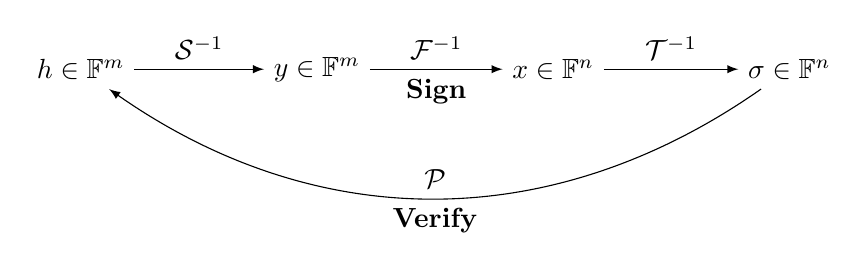
\begin{tikzpicture}
\node (h) at (0, 0) {$h \in \mathbb{F}^m$};
\node (y) at (3, 0) {$y \in \mathbb{F}^m$};
\node (x) at (6, 0) {$x \in \mathbb{F}^n$};
\node (z) at (9, 0) {$\sigma \in \mathbb{F}^n$};
\draw[-latex] (h) -- node[above]{$\mathcal{S}^{-1}$} (y);
\draw[-latex] (y) --
node[above]{$\mathcal{F}^{-1}$} node[below]{\textbf{Sign}} (x);
\draw[-latex] (x) -- node[above]{$\mathcal{T}^{-1}$} (z);
\draw[-latex] (z) to[bend left=35] node[above]{$\mathcal{P}$}
node[below]{\textbf{Verify}} (h);
\end{tikzpicture}
\caption{Flow of the bipolar construction}\label{fig:bipolar}
\end{figure}

The basic construction used in multivariate cryptosystems is based upon the
composition of multiple maps. As in definition \ref{def:mqsystem}, a
multivariate system may be used as a map
$\mathcal{F}:\mathbb{F}^n\to\mathbb{F}^m$. The central map of this construction
will be a map of such kind, which will contain some specific structure such
that one can invert this map. This map will remain secret, and with the
combination of one or more affine maps, a public system of equations, with no
apparent structure, thus hard to solve, will be generated.

As shown in Figure \ref{fig:bipolar}, the bipolar construction consists of
three secret maps, and a public map that is derived from these three.
$\mathcal{P}$ and $\mathcal{F}$ are multivariate systems. $\mathcal{S}$ and
$\mathcal{T}$ are random invertible affine maps. In the signing procedure, one
has to actually invert $\mathcal{F}$ which is not feasible for any multivariate
system, as stated above. Thus, $\mathcal{F}$ introduces some structure that
allows the signer to invert it as the affine maps take care of hiding this
structure by actually scrambling the variables of the system. When generating
the keys one may calculate $\mathcal{P}$ by the composition of the secrete maps
$\mathcal{P} = \mathcal{S} \circ \mathcal{F} \circ \mathcal{T}$.

Note that $n>m$ should hold when using the construction for digital signature
schemes. This makes the public map $\mathcal{P}$ surjective, and ensures that
for every hash $h \in \mathbb{F}^m$ there is a signature $z \in \mathbb{F}^n$.
Encryption schemes can be constructed too, in this case $n < m$ should hold,
thus making the map injective and ensuring that the decryption process outputs
only one plain text. Encryption schemes will not be covered by this work.

With a hash function $\mathcal{H}:\{0,1\}^* \to \mathbb{F}^m$ one can sign a
document $d$ by calculating $h = \mathcal{H}(d)$, then, as shown in Figure
\ref{fig:bipolar}, recursively compute the signature $z =
\mathcal{T}^{-1}(\mathcal{F}^{-1}(\mathcal{S}^{-1}(h)))$. This is possible due
to the fact that those maps are constructed such that they can be inverted. To
verify the signature $z$ for document $d$ one can simply check if $h =
\mathcal{H}(d) = \mathcal{P}(z)$ holds.

\section{Underlying problems}

This section describes the problems in which the multivariate cryptosystems
security rely on.

\subsection{Polynomial system solving}

Solving systems of polynomials is the basic problem, as shown, if it is
feasible to solve the public system, therefore one can forge signatures.

\begin{definition}
Polynomial System Solving problem: given a system $\mathcal{P}$ like the one in
equation \ref{eq:mqsystem}, find a vector $x' = (x_1',\cdots,x_n')$ such that
$p^{(1)}(x') = p^{(2)}(x') = \cdots = p^{(m)}(x') = 0$.
\end{definition}

This problem was proven to be NP-Hard~\cite[Appendix A7.2]{garey1990npc} even
for the simplest case of quadratic polynomials over $GF(2)$. The special case
of this problem where the polynomials have degree 2 is called
\textbf{MQ-Problem}. The NP-Hardness of this problem is important due to the
fact that, it is not feasible for an attacker to solve the public map
$\mathcal{P}$ directly, hence not feasible to forge signatures this way.

\subsection{Isomorphism of polynomials}

The security of multivariate cryptosystems, due to their construction, does not
rely exclusively on the MQ-Problem. An attacker knows that the public map is
constructed by the composition of the private maps, thus one can try to
decompose the map $\mathcal{P}$ into three maps, isomorphic to the private
ones, and forge new signatures. The problem of finding such isomorphic maps is
called Extended Isomorphism of Polynomials problem.

\begin{definition}
Extended Isomorphism of Polynomials problem: given a nonlinear multivariate
system $\mathcal{P} = \mathcal{S} \circ \mathcal{F} \circ \mathcal{T}$ with
$\mathcal{F}$ belonging to some class $\mathcal{C}$ of special nonlinear
systems that can be inverted. Find $\mathcal{S}'$, $\mathcal{F}'$ and
$\mathcal{T}'$ such that $\mathcal{P} = \mathcal{S}' \circ \mathcal{F}' \circ
\mathcal{T}'$ and $\mathcal{F}' \in \mathcal{C}$.
\end{definition}

With $\mathcal{S}'$, $\mathcal{F}'$ and $\mathcal{T}'$ one may forge a
signature to a document $d$ by computing $z =
\mathcal{T}'^{-1}(\mathcal{F}'^{-1}(\mathcal{S}'^{-1}(\mathcal{H}(d))))$ and
publish it as a valid signature for the public key $\mathcal{P}$. Recall that
$\mathcal{F}' \in \mathcal{C}$ so it can be inverted.

Some variations of the problem with less secret maps or even ones that involve
finding the original central map $\mathcal{F}$ exist, but the extended
variation is the most generic one. In fact, solving the problem as stated
above, in polynomial time, is enough to break the Rainbow Signature
Scheme~\cite{ding2005rainbow} submitted to the NIST Post-Quantum Cryptography
Standardization Process.

Opposed to the MQ-Problem, the hardness of this problem is not well
established. Actually, on the balanced Oil and Vinegar
scheme~\cite{patarin1997ov} decomposing the public map was done efficiently by
~\cite{kipnis1998cryptanalysis}. While this problem remains an open problem,
security proofs for multivariate schemes based on the bipolar construction will
be absent. MQDSS\sigla{MQDSS}{Multivariate Quadratic Digital Signature
Scheme}~\cite{chen20165} is a provably secure multivariate cryptosystem,
however it is based on a totally different construction.

\section{Multivariate digital signatures schemes}

This section contains a description of the main schemes that are based on the
bipolar construction.

\subsection{Oil and Vinegar}\label{sec:ov}

The original Oil and Vinegar was presented by \cite{patarin1997ov}, it
introduces a trapdoor that is based upon the idea of having two sets of
variables in the central map, called oil and vinegar. The central map is
constructed in such a way that the polynomials are linear in the oil variables,
that is, there is no monomials that consists of two oil variables. With this
fact in mind, when generating a signature one may actually linearize the
central system and solve for oil variables. A detailed description of the Oil
and Vinegar signature scheme follows.

Let $K$ be a small finite field (\textit{e.g.} $\mathbb{F}_2$). Let $o$ and $v$
be integers, such that $o$ is the number of oil variables and $v$ the number of
vinegar variables. Let $\mathcal{H}: \{0,1\}^* \to K^o$ be a hash function.

The private key consists of two maps $\mathcal{S}$ and $\mathcal{F}$. Let
$\mathcal{S}: K^{o+v} \to K^{o+v}$ be a random \textit{invertible} affine
transformation, this transformation just rewrites every variable as a linear
equation of all other variables. This map will be used to hide the structure of
the central map. Let $\mathcal{F}: K^{o+v} \to K^{o}$ be the central map, this
map is composed of $o$ equations of the form:

\begin{equation}\label{eq:ovpolynomial}
y^{(k)} =
\underbrace{\sum_{i=1}^{v}\sum_{j=i}^{v} \alpha^{(k)}_{ij} x_i x_j}_{
V \times V} +
\underbrace{\sum_{i=v+1}^{v+o}\sum_{j=1}^{v} \beta^{(k)}_{ij} x_i x_j}_{
O \times V} +
\underbrace{\sum_{i=1}^{o+v} \gamma^{(k)}_{i} x_i}_{\text{linear}} +
\underbrace{\delta^{(k)}}_{\text{constant}}
\end{equation}

where $(x_1,\dots,x_v)$ are the ``vinegar'' variables and
$(x_{v+1},\dots,x_{v+o})$ are the ``oil'' variables. Notice that the oil
variables do not multiply themselves, this will be important to make this map
invertible when signing a message.

The public map $\mathcal{P}$ is a simple composition of the secret maps
($\mathcal{P} = \mathcal{F} \circ \mathcal{S}$). Both $\mathcal{F}$ and
$\mathcal{P}$ are multivariate systems. $\mathcal{F}$ has the special structure
mentioned above, nevertheless $\mathcal{P}$ looks randomly built. With this
maps described, let the public/private key pair be
$(\mathcal{P},(\mathcal{S},\mathcal{F}))$.

To sign a document $d$, compute its hash value $h = \mathcal{H}(d)$, find a
preimage $(x_1,\dots,x_{o+v})$ for the map $\mathcal{F}$ such that
$(y_1,\dots,y_o) = (h_1,\dots,h_o)$. Recall the structure present in
$\mathcal{F}$, setting random values to the vinegar variables makes the system
linear. Hence, the signing procedure consists of selecting vinegar variables at
random, substitute them into $\mathcal{F}$ and find the rest of the, oil,
variables through Gaussian elimination. If the system cannot be solved, new
vinegar variables need to be chosen. The set of variables $x$ are found such
that $\mathcal{F}(x)=h$.

Next, using the map $\mathcal{S}$ the signature itself may be computed. Recall
that $\mathcal{S}$ is invertible, thus $\mathcal{S}^{-1}$ can be easily
obtained. With both maps inverted, the signature $\sigma$ of $d$ is published
as $\sigma = \mathcal{S}^{-1}(x)$.

To verify a signature $\sigma$ of a document $d$, one can simply check if
$\mathcal{P}(\sigma) = \mathcal{H}(d)$ holds, therefore the signature is valid,
otherwise it is invalid. The equality does actually hold for valid signatures,
as $\mathcal{P}$ is a composition of the maps that were inverted in the signing
procedure. Although, solving $\mathcal{P}$ is unfeasible. Remind that
$\mathcal{P}$ is a multivariate equations system, hence hard to solve.

\subsection{Unbalanced Oil and Vinegar}

The original Oil and Vinegar explained in section \ref{sec:ov} is actually
insecure due to the fact that $o = v$. It is called Balanced Oil and Vinegar
due the same amount of oil and vinegar variables. This aspect of the
cryptosystem was exploited by~\cite{kipnis1998cryptanalysis}, this work
introduced a method to efficiently forge new signatures when $o = v$. The same
authors subsequently propose a new scheme called Unbalanced Oil and
Vinegar~\cite{kipnis1999unbalanced}. This work proposes new parameters for the
original OV\sigla{OV}{Oil and Vinegar}, the most common instantiation of this
new scheme is the $v = 2o$ case, furthermore a series of other parameters were
mentioned and analysed.

\subsection{Rainbow}

The Rainbow signature scheme was proposed in~\cite{ding2005rainbow}. It can be
described simply as a multilayered OV. Actually, it is a generalization of the
OV scheme, in other words, OV is a single layer Rainbow instantiation. This
newly proposed scheme greatly improves space requirements in comparison to OV.
Both public and private key sizes are reduced for the same security levels, as
well as the signatures size. A detailed description of the Rainbow cryptosystem
follows.

Each layer of this so called Rainbow will have its own polynomials as well as
its own set of oil and vinegar variables. This polynomials will have the same
structure as the OV polynomials, but the layers are intrinsically connected
when constructed. Namely, $V_l$ and $O_l$ are respectively the set of vinegar
variables and the set of oil variables of the $l$-th layer. Let $u$ be the
number of layers. Let $v_1, v_2, \cdots, v_{u+1}$ be the number of vinegar
variables in each layer, such that $0 < v_1 < v_2 < \cdots < v_{u+1} = n$. Note
that the layers actually grow bigger, this is due to the fact that each set of
vinegar variables contains the vinegar variables from the previous layer, that
is $V_1 \subset V_2 \subset \cdots \subset V_{u}$. As you go deeper into the
layers, the oil variables become vinegar variables, \textit{id est} $V_{l+1} =
V_l \cup O_l$. Keep in mind that $|V_l| = v_l$ and $|O_l| = o_l = v_{l+1} -
v_{l}$.

The connection between the variables of the layers exist in such a way that the
layers have to be inverted one after the other for one to completely invert the
central map. To start the inversion of the central map, one randomly selects
the first set of vinegar variables and substitutes them, making the first layer
linear. Recall that the oil variables of some layer are part of the vinegar
variables of the subsequent layer. When the first layer is solved, the set
$O_1$ can be used to construct $V_2$ in its entirety. With known values for
$V_2$ one can linearize the second layer and solve it. Repeating this process
for every layer, inverts the whole central map.

Let the sets $V_l = \{x_1, \cdots, x_{v_l}\}$ be the vinegar variables of the
$l$-th layer and $O_l = V_{l+1} - V_l$ the oil ones. Each layer $l$ has $o_l =
v_{l+1} - v_{l}$ equations due to the fact that $|O_l| = o_l$, hence $o_l$
equations are needed to solve for $O_l$ variables. For each layer $l$,
construct a system $\mathcal{F}_l$ composed of $o_l$ polynomials of the form:

\begin{equation}
y^{(k)} =
\sum_{i=1}^{v_l}\sum_{j=i}^{v_l} \alpha^{(k)}_{ij} x_i x_j +
\sum_{i=v_l+1}^{v_{l+1}}\sum_{j=1}^{v_l} \beta^{(k)}_{ij} x_i x_j +
\sum_{i=1}^{v_{l+1}} \gamma^{(k)}_{i} x_i +
\delta^{(k)}
\end{equation}

for $k = v_l, \cdots, v_{l+1} - 1$ and $l = 1, \cdots, u$. Observe that the
polynomials are Oil and Vinegar polynomials, just like the ones in
equation~\ref{eq:ovpolynomial}, and they can be solved for $O_l$ when $V_l$ has
known values. Let the central map $\mathcal{F}:K^{n} \to K^{n-v_1}$ be the
union of the $u$ layers. To hide the central map, two random affine maps will
be used. Let $\mathcal{S}:K^{n-v_1} \to K^{n-v_1}$ and $\mathcal{T}:K^{n} \to
K^{n}$ be part of the private key. Publish $\mathcal{P} = \mathcal{S} \circ
\mathcal{F} \circ \mathcal{T}$ as the public key.

To sign a document $d$, using a hash function $\mathcal{H}: \{0,1\}^* \to
K^{n-v_1}$, compute $h = \mathcal{H}(d)$. Compute $y = (y_1, \cdots, y_{n-v_1})
= \mathcal{S}^{-1}(h)$. Solve all layers of $\mathcal{F}$, finding $x = (x_1,
\cdots, x_n)$ such that $\mathcal{F}(x) = y$. Finally, publish $\sigma =
\mathcal{T}^{-1}(x)$ as the signature for $d$.

Verifying a signature $\sigma$ for document $d$ is as simples as checking if
$\mathcal{P}(\sigma) = \mathcal{H}(d)$ holds. Recall that, again, $\mathcal{P}$
is a multivariate system that appears to be randomly built, thus hard to solve
directly.

\section{Rainbow variants}

The cryptosystems described above have a notable space requirement. For
instance, the Rainbow public key can get up to 1.6 MB for secure
parameters~\cite{ding2017nist}. This section presents some variants in the
literature that reduce Rainbow key sizes. Notably, all of them reduce either
the public key or the private key, but not both.

\subsection{Establishing a linear relation between public and private maps}
\label{sec:relation}

In~\cite{petzoldt2010cyclicrainbow} an approach is used in such way that one
can partially select the public key. It relies on an important aspect of the
schemes discussed here. On the UOV\sigla{UOV}{Unbalanced Oil and Vinegar} case,
it is appointed that the secret map $\mathcal{S}$ actually establishes a linear
relation between the private and public coefficients of the equations. This
makes it possible to select $\mathcal{P}$ and $\mathcal{S}$ in a smart manner
such that you can actually make their representations smaller, introducing some
kind of structure like a circulant matrix in the case of the CyclicRainbow.

Recall the UOV construction of the maps $\mathcal{P} = \mathcal{F} \circ
\mathcal{S}$. To understand this linear relation, the equations can be
simplified, without its linear and constant terms. Let $n = o + v$, suppose
that the $k$-th private polynomial of the system, without its linear and
constant terms, is denoted like:

\begin{equation}
y^{(k)} = \sum_{r=1}^n \sum_{s=r}^n\left(\alpha^{(k)}_{rs}x_rx_s\right)
\end{equation}

Let $\mathcal{S} \in K^{n \times n}$ be the matrix that describes the secret
affine map. The $k$-th public polynomial can be written as:

\begin{equation}\label{eq:pubpolynomial}
p^{(k)} = \sum_{r=1}^n \sum_{s=r}^n
\left[ \alpha^{k}_{rs} \sum_{i=1}^n(s_{ir}x_i) \sum_{j=1}^n(s_{js}x_j) \right]
\end{equation}

where $s_{ij}$ is the element of $\mathcal{S}$ in the $i$-th line and the
$j$-th column. The summations come from the matrix multiplication operation,
the vector of $x$ variables is actually being multiplied with $\mathcal{S}$
when the map is applied, giving  a ``new'' vector of $x$ variables, that are
actually just linear combinations (the summations) of the old ones. Let's say
we want to describe our public polynomial, just like our private one:

\begin{equation}
p^{(k)} = \sum_{r=1}^n \sum_{s=r}^n \left( \rho^{(k)}_{rs}x_rx_s \right)
\end{equation}

To establish a relation between $\alpha_{rs}$ and $\rho_{rs}$ we need to
observe the structure of equation \ref{eq:pubpolynomial} where $\alpha_{rs}$ is
multiplying two polynomials. We can write those two multiplying polynomials as:

\begin{equation}
(s_{1r}x_1 + s_{2r}x_2 + \cdots + s_{nr}x_n)
(s_{1s}x_1 + s_{2s}x_2 + \cdots + s_{nr}x_n)
\end{equation}

This can be described as a new polynomial with quadratic terms, applying
distributive multiplication:

\begin{equation}\label{eq:tau}
\sum_{i=1}^{n}\sum_{j=i}^n \left( \tau^{rs}_{ij} x_i x_j \right)
\end{equation}

where:

\begin{equation*}
\tau^{rs}_{ij} =
\begin{cases}
	s_{ir} s_{is} &\mbox{if } i=j \\
	s_{ir} s_{js} + s_{jr} s_{is} &\mbox{otherwise}
\end{cases}
\end{equation*}

Substituting \ref{eq:tau} into \ref{eq:pubpolynomial} we get:

\begin{equation}
p^{(k)} = \sum_{r=1}^n \sum_{s=r}^n
\left[
\alpha^{k}_{rs} \sum_{i=1}^{n}\sum_{j=i}^n \left( \tau^{rs}_{ij} x_i x_j \right)
\right]
\end{equation}

Therefore, a relation between private and public coefficients can be written as:

\begin{equation}\label{eq:relation}
\rho^{(k)}_{ij} = \sum_{r=1}^{n}\sum_{s=r}^n
\left( \tau^{rs}_{ij} \alpha^{k}_{rs} \right)
\end{equation}

After we randomly choose $\mathcal{S}$, equation \ref{eq:relation} depicts the
linear relation between the public ($\rho$) and private ($\alpha$)
coefficients, hence we could either choose and fix $\rho$ or $\alpha$ and find
the other using this equation. We need to observe that we cannot choose all
public coefficients to achieve the structure in $\mathcal{F}$. This could also
be used to recalculate $\mathcal{F}$ from $\mathcal{P}$ and $\mathcal{S}$, this
will be important later. The idea behind this relation can be further expanded
to Rainbow key pairs, such relation is described in detail
by~\cite{petzoldt2011small}. This relation was extensively used to reduce
public keys or private keys, but not both. Reducing key sizes in this manner
consists of introducing some structure into one part of the key, such that its
representation becomes smaller, and calculating the other part using the
equations above. Notable key optimizations will be briefly discussed hereafter.

% rainbow variants

%% smaller public keys

\subsection{CyclicRainbow}

CyclicRainbow~\cite{petzoldt2010cyclicrainbow} uses the relations explained in
section~\ref{sec:relation} to structure the public key. In the key generation
step, parts of the public key matrix representation are selected such that they
form a circulant matrix. An $n \times n$ circulant matrix is of the form:

\begin{equation}
A =
\begin{pmatrix}
a_1     & a_2    & \cdots  & a_{n-1} & a_n     \\
a_n     & a_1    & a_2     & \cdots  & a_{n-1} \\
a_{n-1} & a_n    & a_1     &         & a_{n-2} \\
\vdots  &        & \ddots  & \ddots  & \vdots  \\
a_2     & \cdots & a_{n-1} & a_n     & a_1
\end{pmatrix}
\end{equation}

Such matrices allow for a compact representation. Storing the vector $(a_1,
a_2, \cdots, a_n)$ is enough to represent the matrix completely, as its
elements depict a structured repetition. Introducing this structure in parts of
the public key, when possible, reduces the representation of the public system
significantly. In fact this method allows a public key reduction factor of up
to 2.9, for secure parameters. This repetition of elements also leads up to a
repetition of operations when verifying a signature. Exploiting this common
field multiplications leads to a reduction factor of up to 2.4 in the number of
operations needed to evaluate the public map, \textit{i.e.} to verify a
signature \cite{petzoldt2013thesis}.

\subsection{RainbowLRS2}

RainbowLRS2~\cite{petzoldt2013thesis} introduces matrices generated by Linear
Recurring Sequences into the public key, just like in CyclicRainbow. To
generate an $m \times n$ matrix of this type, a vector $a = (a_1, a_2, \cdots,
a_m) \in \mathbb{F}_q^m$ of distinct elements is selected. The $i$-th row of
this matrix is:

\begin{equation}\label{eq:lrsmatrix}
A[i] = (a_i^0, a_i^1, a_i^2, \cdots, a_i^{n-1}) \qquad i = 1, \cdots, m
\end{equation}

Keeping the vector $a$ is sufficient the represent the matrix $A$, as all its
rows can be calculated using equation \ref{eq:lrsmatrix}. Using matrices of
this fashion in the public map representation, allows for a reduction factor of
up to 3.1. Veritably, this method is pretty much similar to the one used in
CyclicRainbow, thus provides an akin improvement in space requirements. The
main difference is that CyclicRainbow uses rotations to generate each row. In
RainbowLRS2 the rows are defined by equation \ref{eq:lrsmatrix}. It is shown
in~\cite{petzoldt2013thesis} that field multiplications also repeat in the
verification process of RainbowLRS2, which allows for a speed up to a factor of
2.2.

%%% other non-Petzoldt variants

%% smaller private keys

%%% Lite Rainbow

%%% Efficient variant of Rainbow using sparse secret keys

%%% Efficient variant of rainbow without triangular matrix representation

\chapter{Diminishing key pairs by fixing vinegar variables}

\chapter{Conclusion}

\bibliographystyle{abnt-alf}
\bibliography{ref}

\end{document}
